\documentclass[tikz,border=6pt]{standalone}
\usepackage{amsmath}
\usetikzlibrary{arrows.meta,calc,patterns,positioning}
\begin{document}

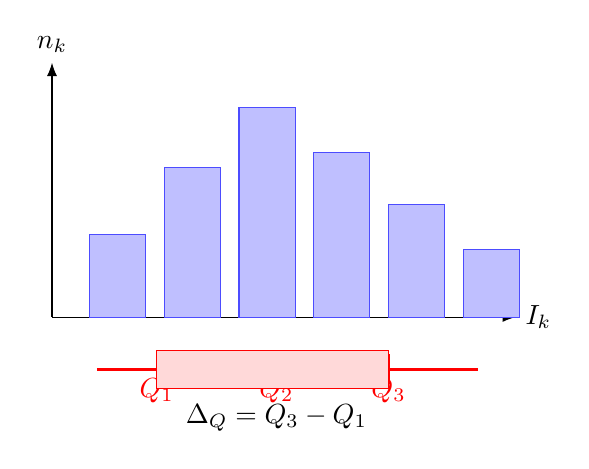
\begin{tikzpicture}[>=Latex,scale=0.95]
  \draw[->] (0,0) -- (6.2,0) node[right] {$I_k$};
  \draw[->] (0,0) -- (0,3.4) node[above] {$n_k$};
  \foreach \x/\h in {0.5/1.1,1.5/2.0,2.5/2.8,3.5/2.2,4.5/1.5,5.5/0.9} {
    \draw[fill=blue!25,draw=blue!70] (\x,0) rectangle +(0.75,\h);
  }
  \draw[thick,red] (0.6,-0.7) -- (5.7,-0.7);
  \draw[thick,red] (1.4,-0.9) -- (1.4,-0.5) node[below=5pt] {$Q_1$};
  \draw[thick,red] (3.0,-0.9) -- (3.0,-0.5) node[below=5pt] {$Q_2$};
  \draw[thick,red] (4.5,-0.9) -- (4.5,-0.5) node[below=5pt] {$Q_3$};
  \draw[fill=red!15,draw=red] (1.4,-0.95) rectangle (4.5,-0.45);
  \node at (3,-1.35) {$\Delta_Q=Q_3-Q_1$};
\end{tikzpicture}

\end{document}
